% section 2: Components

\section{Components}\label{sComp}

\subsection{Application Structure}
The production DMS (as described in our reference 
design\footnote{http://dev.lsstcorp.org/model/LSSTModel.pdf}) will
contain three pipeline-processing systems which we refer to as
\textit{multi-pipelines}.  A multi-pipeline is a set of one or more
loosely-coupled pipelines that coordinate to create a set of related
data products.  The three multi-pipelines, illustrated in
\Fig{fComp-pipe}, divide their responsibilities between nightly
processing, calibration products, and data release processing.  DC2 is
intended specifically to prototype the nightly processing pipeline.
The full structure of this pipeline as intended for the production DMS
is shown in more detail in \Fig{fComp-nite}.  DC2 implements
the ``backbone'' of the nightly processing flow; illustrated in
\Fig{fComp-dc2}, it includes:

\begin{itemize}
\item Image subtraction;
\item Source detection;
\item Association of Sources to Objects; and
\item The ``night'' portion of the Moving Objects Prediction Software
  (MOPS), which calculates predicted positions of known solar system
  objects in the incoming exposures.
\end{itemize}

As can be seen in part from a comparison of \Fig{fComp-nite} and
\Fig{fComp-dc2}, several aspects of the full LSST nightly processing were
not included in DC2: 

\begin{itemize}
\item Instrumental signature removal stage of the image processing
  pipeline (debiasing, flatfielding, etc.);
\item Alert processing;
\item The ``day'' portion of MOPS, which links together detections
  into tracks, and determines orbits; and
\item Combined processing of the two exposures which make up a single
  visit. The DC2 input data (\Sec{sInDat}) was not taken with the
  required cadence to allow this.
\end{itemize}

\begin{figure}[htbp]
\begin{center}
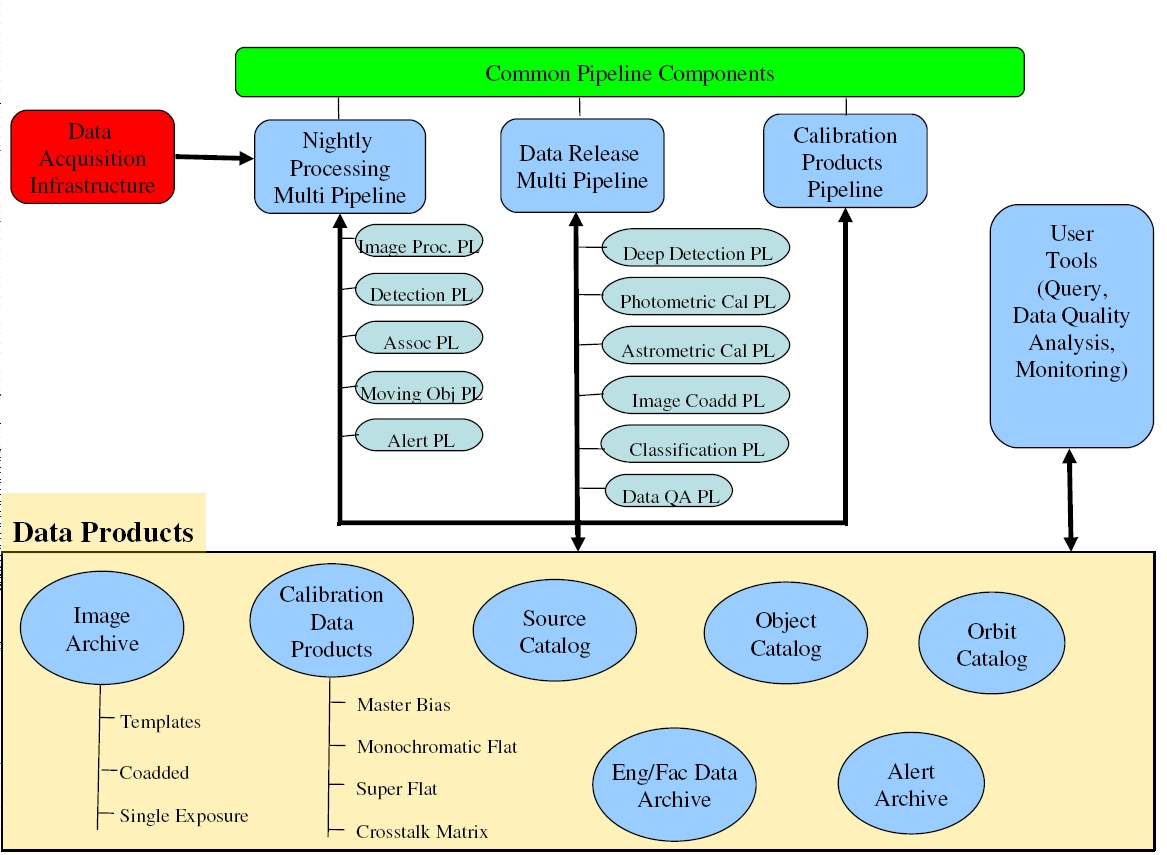
\includegraphics[height=0.45\textheight] {figures/LSSTPipelines}
\caption{The LSST Data Management Pipelines\label{fComp-pipe}}
\end{center}
\end{figure}

\begin{figure}[htbp]
\begin{center}
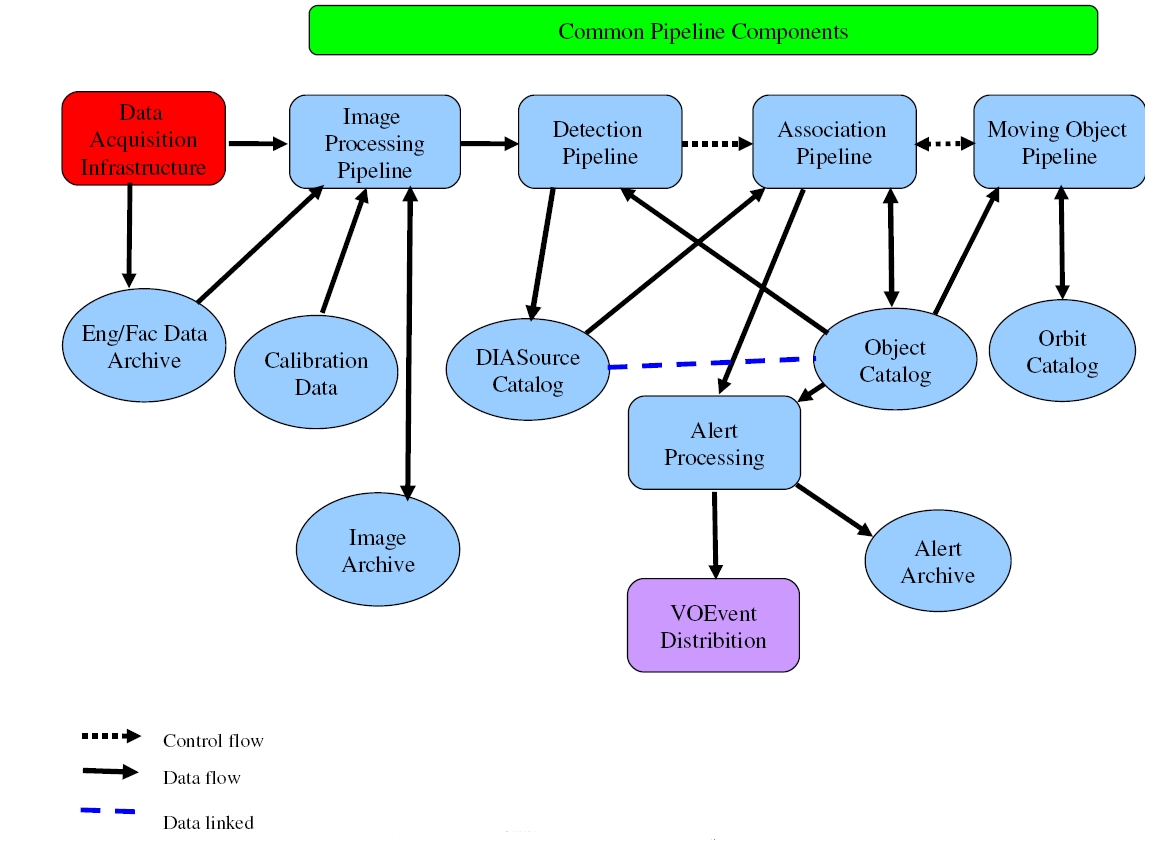
\includegraphics[height=0.45\textheight] {figures/LSSTNightlyPipeline}
\caption{The LSST Nightly Pipelines\label{fComp-nite}}

\vspace{0.05\textheight}

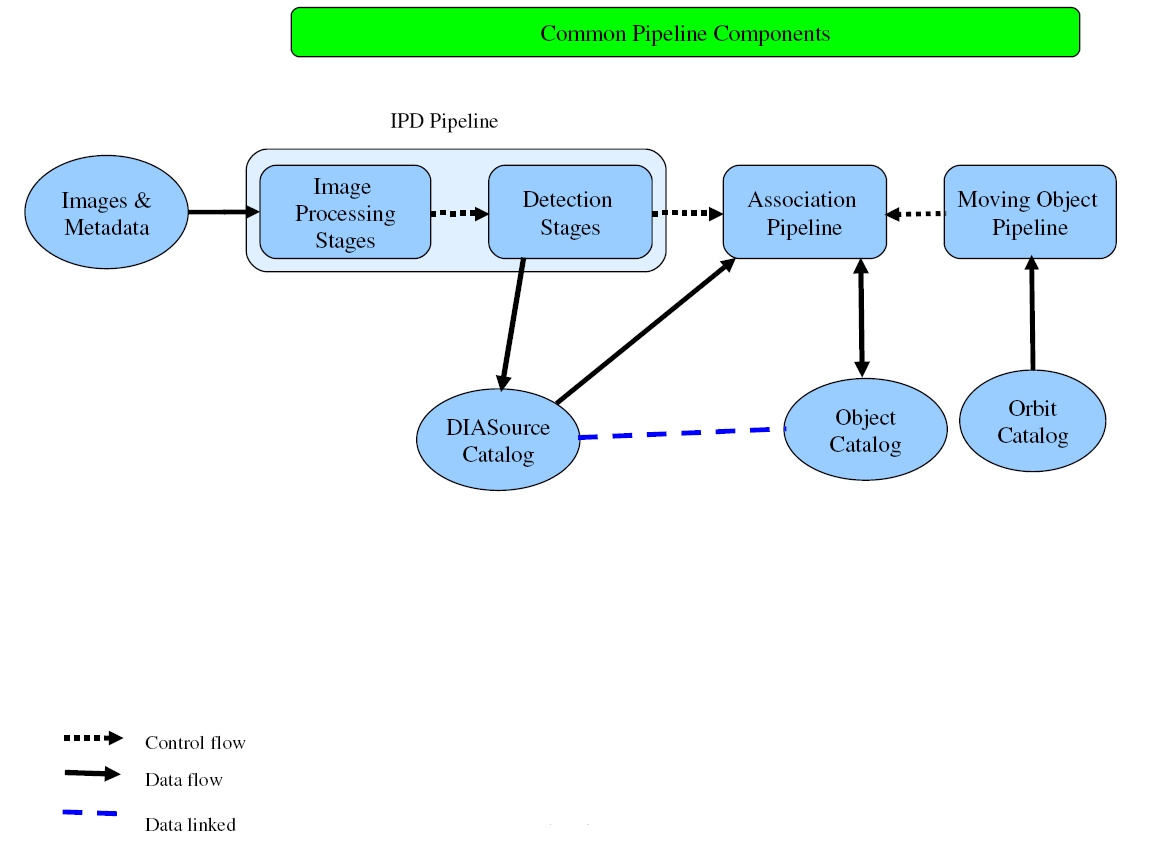
\includegraphics[height=0.45\textheight] {figures/DC2Pipelines}
\caption{The DC2 Pipelines\label{fComp-dc2}}
\end{center}
\end{figure}

The DC2 system is functionally comprised of three separate pipelines:
the Image Processing and Detection (IPD) pipeline, the Moving Object
(MOPS) pipeline, and the Association pipeline.  (Although the Image
Processing and Detection pipelines are logically separate pipelines in
our design, we have implemented them in our software framework as
stages within a single functional pipeline.  This choice does not
change the logic of the applications flow, but increases the execution
efficiency, since the images being transferred between Image
Processing and Detection can remain in memory without consuming I/O
resources.)  The three pipelines are loosely coupled via event-based
communication (\Sec{sMw-ev}).  They also share access to a
MySQL\footnote{http://www.mysql.com} database.  An early prototype of the pipeline
orchestration layer (\Sec{sMw-orc}) is responsible for deploying
the multi-pipeline to a cluster, executing it, and feeding it its
input data.  The whole system is configured via a set of so-called
\textit{policy files}.  These define the different stages that make up
the pipelines and provide values for parameters that control the behavior
of components.

\subsection{Summary of Processing Flow}\label{sComp-flo}

The DC2 multi-pipeline is executed via the orchestration layer
(\Sec{sMw-orc}) which is represented by the \code{dc2pipe} software
package.  Before actually starting the pipelines, the operator usually
configures the pipeline by making a copy of the default policies for
the particular flavor of pipeline being run (found in a repository
that is part of the \code{dc2pipe}) and then altering the values as
desired.  Among the configuration parameters that can be set are the machines that
will be used, the number of parallel processes that will be employed,
and the subset of CCDs making up each observed mosaic that should be
processed.  A separate file lists the sequence of exposures (which we
refer to as \textit{visits}) that the pipelines will operate on.
Normally, the operator uses one of a few default lists provided by the
\code{dc2pipe} package, but the file can be altered as desired.

\begin{table}[htbp]
\begin{center}
\caption{Summary of the stages composing the nightly pipelines\label{tComp-stg}}
\vspace{\baselineskip}
\begin{tabular}{|cp{0.85\textwidth}|}
\tableline
\multicolumn{2}{|l|}{Image Processing and Detection (IPD)} \\
  1 & Create links to the visit's input images in the run's filesystem 
      sandbox. \\
  2 & Load the visit's input images into memory. \\
  3 & Transform the visit's metadata. \\
  4 & Record the visit's metadata in the database. \\
  5 & Write out a copy of the input image data. \\
  6 & Subtract the input images. \\
  7 & Write out the difference image. \\
  8 & Detect sources in the difference image. \\
  9 & Record the detected sources into the database's DIASource catalog. \\
 10 & Send an event to the association pipeline indicating that
      detections are ready. \\
\tableline
\multicolumn{2}{|l|}{Moving Object Processing (MOPS)} \\
  1 & Load visit-specific data into memory.  (Currently no such data
      is being loaded.) \\
  2 & Predict the locations of known moving objects in the field. \\
  3 & Record the predicted positions into the database. \\
  4 & Send an event to the association pipeline indicating that
      predictions are available. \\
\tableline
\multicolumn{2}{|l|}{Association} \\
  1 & Load the Object catalog for the relevant sky region into memory. \\
  2 & Load new source detections from the DIASource catalog into memory. \\
  3 & Match the detections against known, non-moving objects. \\
  4 & Record matched sources into the database.  \\
  5 & Load new MOPS predictions into memory. \\
  6 & Match the detections against known, moving objects.  \\
  7 & Record the matched sources into the database.  \\
  8 & Update historical knowledge of the sky.  \\
\tableline
\end{tabular}
\end{center}
\end{table}

Once the system is configured, the operator starts it via a script 
(\code{launchDC2.py}) which deploys the pipelines on the proper
machines.  One important input to this script is an identifier
referred to as a \textit{run-ID}.  This is used to set up ``sandboxes''
on the file system and in the database where data related to this
particular execution --- or \textit{run} --- of the pipeline can be collected
and kept separate from other pipeline runs.  After the sandboxes are
set up, the pipeline processes are started on the proper machines which,
after some initialization, pause to await the arrival of new data to
process.  

New data is sent to the pipelines by the orchestration layer via a
sequence of event messages.  These messages are constructed in DC2 from
the information found in the file containing the list of visits, a
role that will be played by the Camera data acquisition interface on
the production LSST.  For
each visit, the information includes a visit identifier, the filter
that was used during the visit, and the sky position for the center of
that field.  The visit events are delivered in sequence to both the
IPD and MOPS pipelines, and the first stage of each processes them in
order.  The MOPS pipeline uses the field position to calculate the
predicted positions within the field of known moving objects.  The IPD
uses the visit information to find the next calibrated exposure along
with the associated template images and load them into memory.  

Each pipeline is composed of a sequence of \textit{stages}
(\Sec{sMw-har}).  Data are passed through the stages via a set of 
data queues that stitch the stages together.  Pipelines can coordinate
their activities by sending and receiving event messages.
Table~\ref{tComp-stg} summarizes the function of each stage in each of the
three pipelines.  

In summary, the IPD pipeline first loads the input images into memory.
It next applies the image subtraction algorithm (\Sec{sApp-imsub}) to
produce a difference image.  The detection stage then extracts sources
present in the difference image; these sources represent new objects,
objects that vary in brightness, moving objects, or possibly artifacts
such as cosmic rays.  Descriptions of
these detected sources are stored in the DIASource catalog within the
database.   At the end of the IPD pipeline, it sends an event to the
Association pipeline to tell it that new source detections are
available in the database.  The IPD pipeline then returns to its first
stage and begins operating on the next visit in the input queue.

Meanwhile, as the IPD is processing a visit, the MOPS processes the
same visit in parallel.  It uses the Orbit Catalog to predict the
positions of known moving objects that should appear in the visit's
field of view at the time of its observation.  These predicted
positions are also stored in the database.  The last stage of the
pipeline sends an event to the Association pipeline indicating that
the predicted positions are available.  The MOPS pipeline then returns
to its first stage to process the next field of view.   

The Association pipeline first waits for the event from the IPD
pipeline indicating that new source detections are available for
processing.  It reads the detections from the database and tries to
match them against known (stationary) objects in the Object Catalog.
For those sources that do not yet match known objects, the Association
pipeline uses the event from the MOPS pipeline to match them against
known moving objects.  The DIASource and Object catalogs are updated
to record the matched and unmatched source detections.  At this point, 
the nightly processing for a visit is complete.  

\subsection{The Deployment of DC2 onto Hardware}\label{sComp-hw}

The DC2 pipelines ran on a small, dedicated cluster located at NCSA
comprised of ten Dell Server blades with Xeon processors.  Four of the
blades are of an older model acquired from a past project and
featuring an earlier model processor with fewer cores per node than
the rest of the cluster; the remaining six are identical blades
feature dual, quad-core processors.  \Table{tComp-hw} summarizes
the processor configuration for the ten nodes.  All the nodes feature
4 GB of RAM except node 10, which has 16 GB.  This node was configured
to host the database, which needs the extra memory for handling very
large tables.  All nodes run 32-bit Red Hat Enterprise Linux AS
Release 4. 

Each node features a modest amount of local disk to hold the OS with
about $~50$ GB available potentially for storing local pipeline data.
Node 10 features a locally-mounted 280 GB filesystem for storing the
database data.  Approximately 750 GB of SAN-based storage (with
optical fiber connects) are available as shared, cross-mounted
filesystems (i.e.~available to all nodes), hosting the LSST software
stack, the repository of input data, and the pipeline run sandboxes.
Originally, this was mounted as a Lustre filesystem, providing
redundant, parallel I/O capabilities to the pipeline.  In this
configuration, the older nodes 1--4 were set up to be used exclusively
as file server nodes.  However, our deployment of the Lustre
filesystem proved unstable, and we were forced to replace this with an
NFS-mounted filesystem.  The expected performance penalties for
NFS did appear
to affect the overall performance of the pipelines, particularly in 
the Association pipeline.

\begin{table}[tb]
\begin{center}
\caption{Hardware summary for the DC2 cluster\label{tComp-hw}}
\begin{tabular}{ccccl}
%\multicolumn{5}{c}{Table \ref{tComp-hw}.  Hardware summary for the DC2 cluster}\\
\multicolumn{5}{c}{\phantom{Hardware summary for the DC2 cluster}}\\
\tableline\tableline
Node & No. of processors & Cores per processor & Memory (GB) & Pipeline hosted \\
\tableline
 1  & 2 & 2 & 4 & IPD \\
 2  & 2 & 2 & 4 & \textit{unavailable}\tablenotemark{a} \\
 3  & 1 & 2 & 4 & \textit{unavailable}\tablenotemark{a} \\
 4  & 1 & 2 & 4 & IPD \\
5-8 & 2 & 4 & 4 & IPD \\
 9  & 2 & 4 & 4 & MOPS \\
 10 & 2 & 4 &16 & Association \\
\tableline
\\[0.5\baselineskip]
\multicolumn{5}{p{0.85\textwidth}}{$^{\rm a}$Hardware and system configuration
  issues made these nodes too unstable for consistent use as pipeline nodes.}\\
\end{tabular}
\end{center}
\end{table}

As shown in Table~\ref{tComp-hw}, the three pipelines were completely
segregated on different sets of nodes.  (The segregation is actually a
constraint imposed by our use of MPI.)  Because of its heavy use of
the database, the Association pipeline was deployed onto node 10.
Though this pipeline is singly-threaded, the remaining compute 
resources were reserved for use by database processes.  The MOPS
pipeline ran with 4 total processes on node 9.  The remaining
available nodes were used to host the IPD pipeline; one process per
available processing core was deployed on each node.  

